\documentclass[conference]{IEEEtran}
% \IEEEoverridecommandlockouts
% The preceding line is only needed to identify funding in the first footnote. If that is unneeded, please comment it out.
\usepackage{cite}
\usepackage{amsmath,amssymb,amsfonts}
\usepackage{algorithmic}
\usepackage{graphicx}
\usepackage{textcomp}
\usepackage{xcolor}
\def\BibTeX{{\rm B\kern-.05em{\sc i\kern-.025em b}\kern-.08em
    T\kern-.1667em\lower.7ex\hbox{E}\kern-.125emX}}

% Definiciones propias
\usepackage{comandos}

\begin{document}

\title{
Tractography ML  \\
{\footnotesize Medical statistics proposal for 2022 Wolfram summer school}
}

\author{
    \IEEEauthorblockN{Armando Benjamín Cruz Hinojosa}
    \IEEEauthorblockA{
        \textit{Universidad Nacional Autónoma de México}\\
        Mexico City, Mexico \\
        aleph\_g@ciencias.unam.mx
    }
}

\maketitle

\begin{abstract}
    Tractography is an MRI technique to estimate white matter structure. Thousands of streamlines are generated and need to be filtered for medical research and insight. The objective of this proposal is to migrate into Wolfram language a machine learning project based on supervised learning to segment tractograms into most common brain structures.
\end{abstract}

%
% Introduction
%
\section{Introduction}
Tractography is a 3D computational modeling technique that statistically estimates white matter fiber paths on the human brain, using magnetic resonance imaging. The results are arrays of three dimensional trajectories called tractograms fig~\ref{tractogram}, that can be used to recreate the brain's connection structure in order to understand its functionality and infer the presence of diseases.

\begin{figure}[htbp]
    \centerline{
        \scalebox{.48}{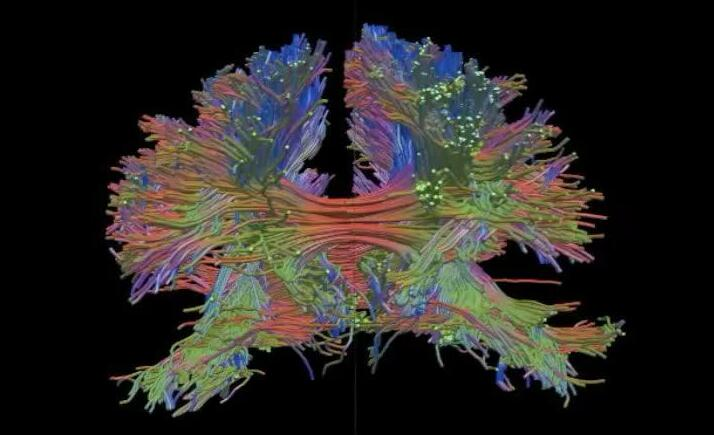
\includegraphics{tractogram.jpg}}
    }
    \caption{Tractogram, tractography algorithms main output.}
    \label{tractogram}
\end{figure}

Due to resolution limitations, a tractogram of a brain cannot obtain individual axons, but clusters of axons. Nevertheless each tractogram contains thousands of clusters that cannot be processed and filtered for medical research without the help of computers.

The task of determining which clusters are connected in the patient's brain is not a trivial task since the fibers overlap and the complex structures of the brain's regions. Because of this, all tractography techniques make mistakes and generate noisy tractograms with many false positive connections.

Solutions to this problem, based on supervised and unsupervised ML algorithms has been proposed such as random forest models, recurrent NN, convolutional NN and auto-encoders. To date, none of these methods have shown conclusive performance or have been established as a main methodology to follow in the field of tractography.

Last summer I had the opportunity to attend the \textit{Summer in mathematical tools for data science}, given at Mexican mathematical research center CIMAT. Over one month a team of six students, one instructor and one neurologist (which I was part of) worked on the implementation of four ML proposals in python, to extract of a given tractogram the main brain structures.

The training data was curated by Dr. Luis Concha from the institute of neurology UNAM. From the four models only two were finished, and one correctly trained with satisfactory results. The project came to be named \textit{Tractosplit} and is allocated in a public github repository \cite{b1}.

%
% Objective
%
\section{Objective}
My proposal is to migrate Tractosplit machine learning project from python into wolfram language. The new code will implement current tractogram segmentation models and the two unfinished models into an instant API running in Wolfram cloud. Additionally implement a 3D interactive plotting of the segmented results, inspired on Muhammad Ubadah's last year Wolfram summer school project \cite{b2}.

%
% Implementation
%
\section{Implementation}
Three things are needed to successfully migrate tractosplit and implement 3d interactive plotting.

\subsection{Training}
Current data for training is the previously mentioned curated data of 30 patients. Each tractogram streamline is assigned a label of the brain section it belongs to, making it ideal for supervised learning models.

More data can be obtained online from the \textit{International Neuroimaging Data-sharing Initiative} \cite{b3} data sets. INDI data sets came from a variety of patients and are curated to study specific diseases like ABIDE: Autism Brain Imaging Data Exchange \cite{b4}.

\subsection{Model definition}
Tractosplit models are a collection of supervised learning architectures whose inputs are tractogram streamlines of size $k\in\{16, 32, 64\}$ ($k$ must be fixed) and return one of 23 labels corresponding to the standard spaces used by XTRACT \cite{b4} tractography tool. Current working architectures are

\begin{itemize}
    \item Long short term memory neural network. This network was proposed by team's instructure Phd. Jean-Bernard Hayet, due to its proficiency on pedestrian trayectory prediction.
    \item Autoencoder.
\end{itemize}
The unfinished models are based on
\begin{itemize}
    \item Random forest. 3D random forest can be represented as a box segmented by prismatic sections (3-cells), calculus theorems assert that all brain sections can be approximated with such prisms.
    \item Convolutional neural network. \cite{b5} propose a CNN based clasifier that successfully identifies 99\% of fibers on average.
\end{itemize}

\subsection{3D interactive plotting}
As mentioned above, segmentation models outputs are a list of several tractogram files, composed of a list of lists size $k\in \{16, 32, 64\}$ of 3D points in brain space.

Each tractogram $k$-list will be plotted as a trajectory in 3d space, and assigned a color depending on the brain section it belongs. Interactivity controls will allow the user to move the 3D camera around the brain and focus on specific brain section.

\newpage
%
% Bibliografía
%
\begin{thebibliography}{00}
    \bibitem{b1} CIMAT’s 2021 Summer in mathematical tools for data science, Brain connectivity team. (2021, June 24). GitHub - Aleph-GORY/tractosplit: Automatic tractography classifier. GitHub. https://github.com/Aleph-GORY/tractosplit

    \bibitem{b2} Ubadah Tanveer, M. (2021, June 20). [WSS21] Biomechanical model of joint movements in human body - Online Technical Discussion Groups—Wolfram Community. Wolfram Community. https://community.wolfram.com/groups/-/m/t/2312437

    \bibitem{b3} International Neuroimaging Data-sharing Initiative. (n.d.). International Neuroimaging Data-sharing Initiative. https://fcon\_1000.projects.nitrc.org/

    \bibitem{b4} FSL. (n.d.). XTRACT - FslWiki. \\https://fsl.fmrib.ox.ac.uk/fsl/fslwiki/XTRACT

    \bibitem{b5} Zhang, F., Cetin Karayumak, S., Hoffmann, N., Rathi, Y., Golby, A. J., \& O’Donnell, L. J. (2020). Deep white matter analysis (DeepWMA): Fast and consistent tractography segmentation. Medical Image Analysis, 65, 101761. https://doi.org/10.1016/j.media.2020.101761

    \bibitem{b6} Hagmann, P., Kurant, M., Gigandet, X., Thiran, P., Wedeen, V. J., Meuli, R., \& Thiran, J. P. (2007). Mapping Human Whole-Brain Structural Networks with Diffusion MRI. PLoS ONE, 2(7), e597. https://doi.org/10.1371/journal.pone.0000597

    \bibitem{b7} Jones, D. K., PhD. (2011). Diffusion MRI. OUP USA.
\end{thebibliography}

\end{document}
